\subsection{Iteration \#3}
I iteration 3 arbejdes med blokke som skal håndterer hvordan der tages billeder, forsendelse af billeder og billede visning. Der monteres kamera på dronen, så den under flyvning kan tage billeder ved de GPS lokationer som bruger har defineret i flyveopsætningen. Alle billeder der tages under flyvning sendes via mobilnet fra dronen til server. Websiden henter automatisk de seneste billeder fra serveren og gør disse tilgængelige for bruger. Hvordan systemet er tiltænkt at bruges beskrives i user story nedenfor:

\subsubsection*{User story}
Under flyvning tager dronen billeder som sendes via 3G/GPS modulet til serveren. Websiden kontrollerer løbende hvilke billeder der er findes på serveren og gør disse tilgængelig for bruger. Login er påkrævet før bruger kan få lov at se billeder fra forskellige flyvninger. Efter succesfuld login på websiden vælger bruger historik og vises information fra tidligere flyvninger. 

%kommentar
\begin{figure}[H]
	\centering
	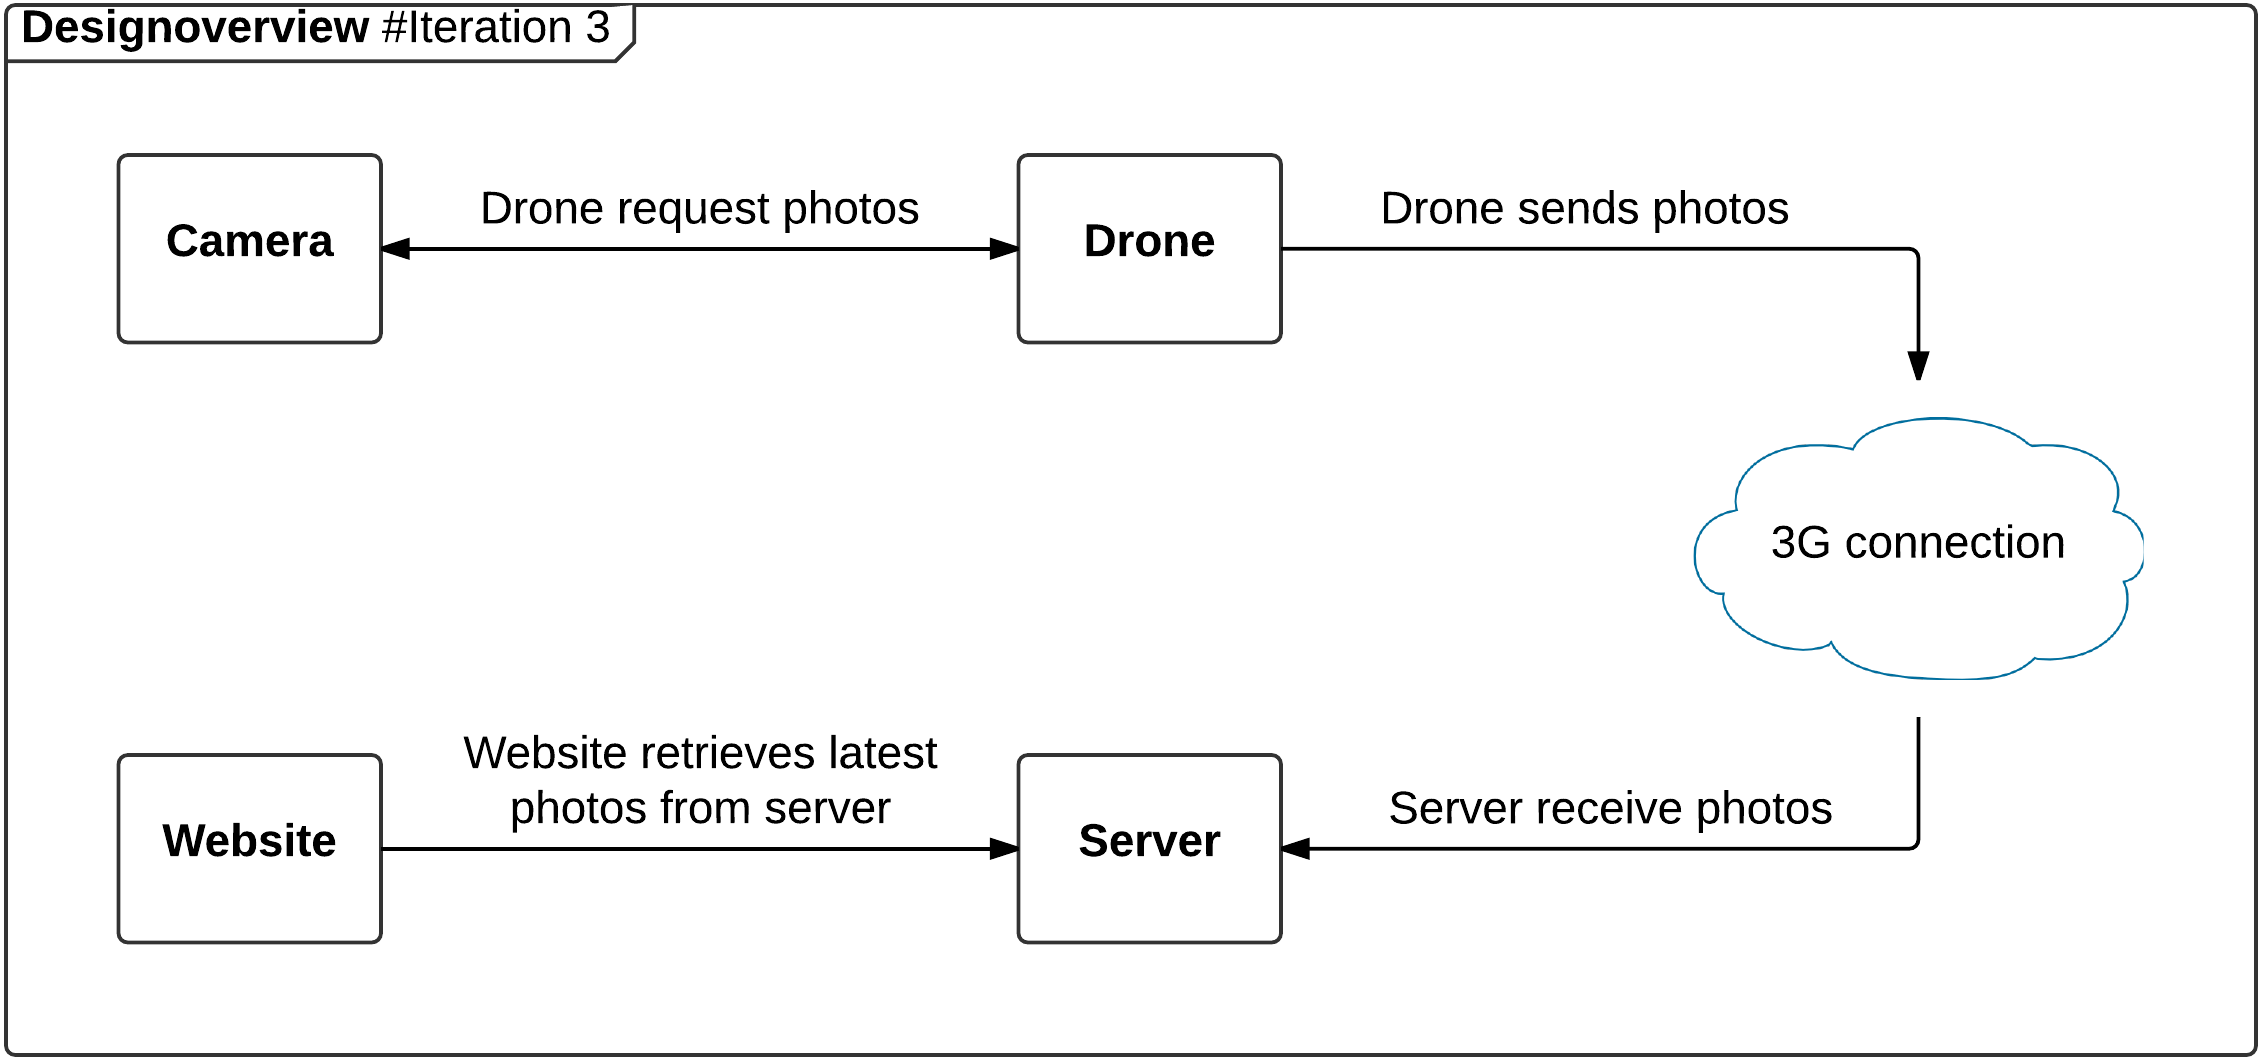
\includegraphics[width=1\textwidth]{Billeder/design_overview/design_overview_iteration3.png}
	\vspace{-.5cm}
	\caption{Designoverview \#iteration 3}
	\label{fig:design_overview_UC1}
\end{figure}
\newpage


\subsubsection*{Sekvens diagram}
\vspace{-0.3cm}
På sekvensdiagrammet på figur \ref{fig:Sekvens_diagram_iteration3}, vises hvilke klasser der indgår og bruges i tredje iteration. På sekvensdiagrammet vises det hvordan kamera delen af 3G/GPS modulet håndteres og hvordan ny tagede billeder sendes med post request til serveren. 

\vspace{-0.2cm}
%kommentar
\begin{figure}[H]
	\centering
	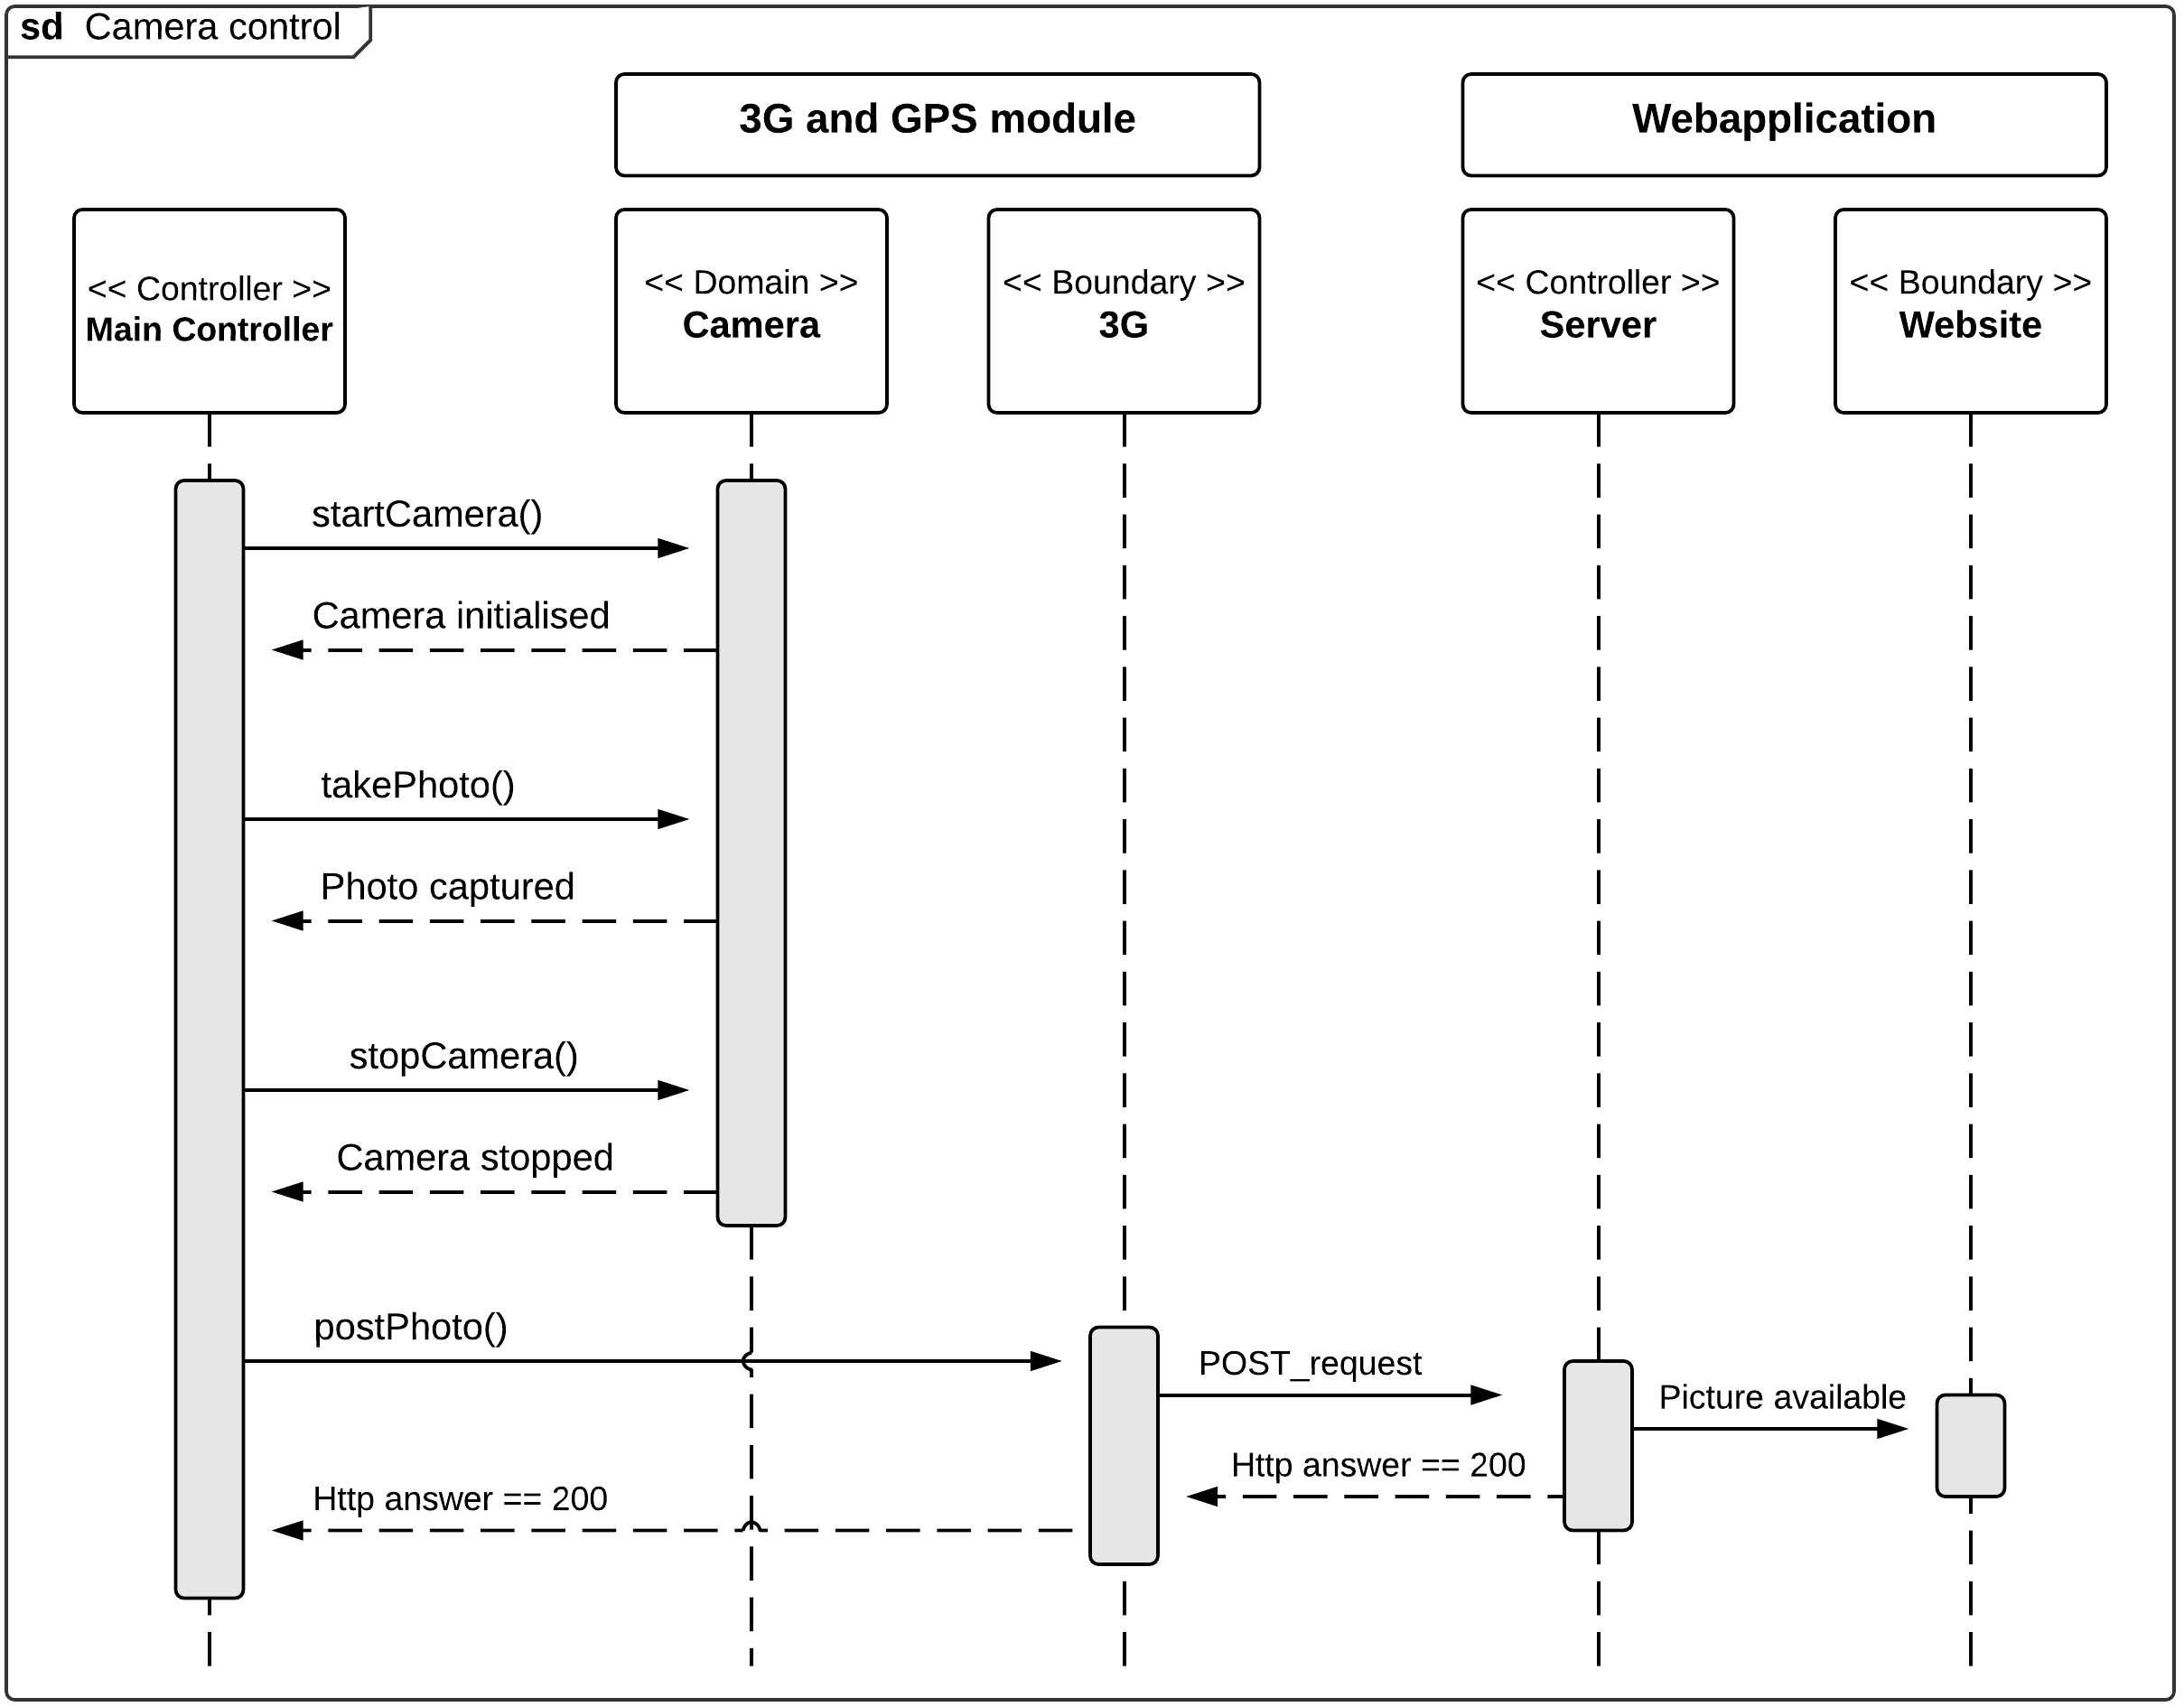
\includegraphics[width=1\textwidth]{Billeder/sekvens/sekvens_iteration3}
	\caption{Sekvens diagram \#iteration 3}
	\label{fig:Sekvens_diagram_iteration3}
\end{figure}
\vspace{-0.2cm}

\subsubsection*{State machine diagram}
\vspace{-0.3cm}
I state machine diagrammet på figur \ref{fig:Statemachine_iteration3}, vises de to states der eksisterer i iteration 3 og hvordan flowet imellem dem ser ud. Der eksisterer givet vis kun 2 states i iteration 3, men state machinen er medtaget fordi den fint illustrerer systemflowet.

\vspace{-0.2cm}
%kommentar
\begin{figure}[H]
	\centering
	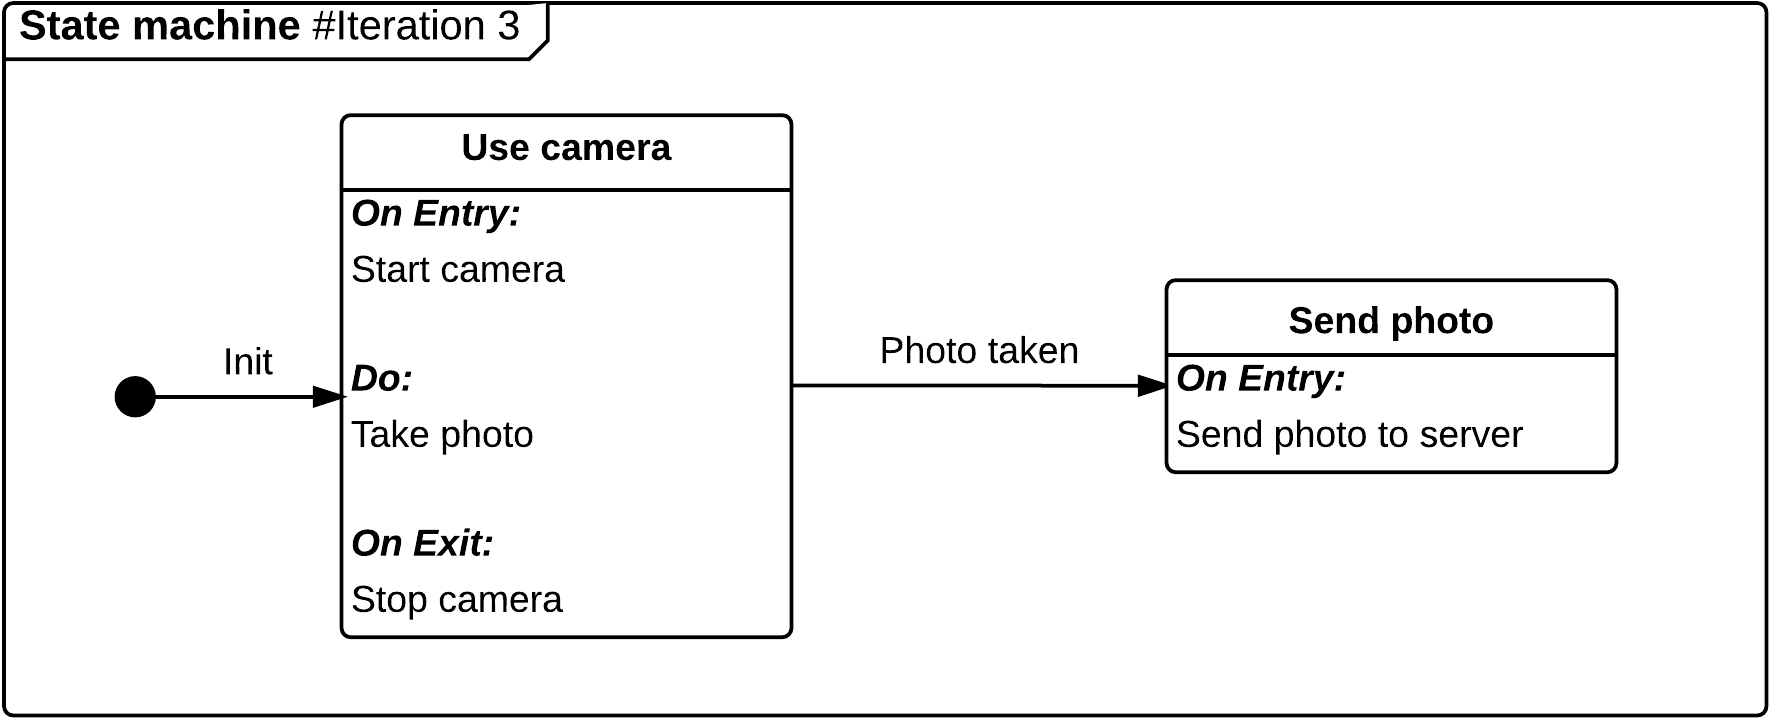
\includegraphics[width=0.9\textwidth]{Billeder/statemachine/State_iteration3.png}
	\caption{State machine \#iteration 3}
	\label{fig:Statemachine_iteration3}
\end{figure}


\subsubsection*{Klasse diagram}

Figur \ref{fig:classDiagram_iteration3} vises et klassediagram tilhørende iteration 4. Klassediagrammet viser foruden main.cpp filen iteration 4's eneste centrale klasse og dens tilhørende metode. 

%kommentar
\begin{figure}[H]
	\centering
	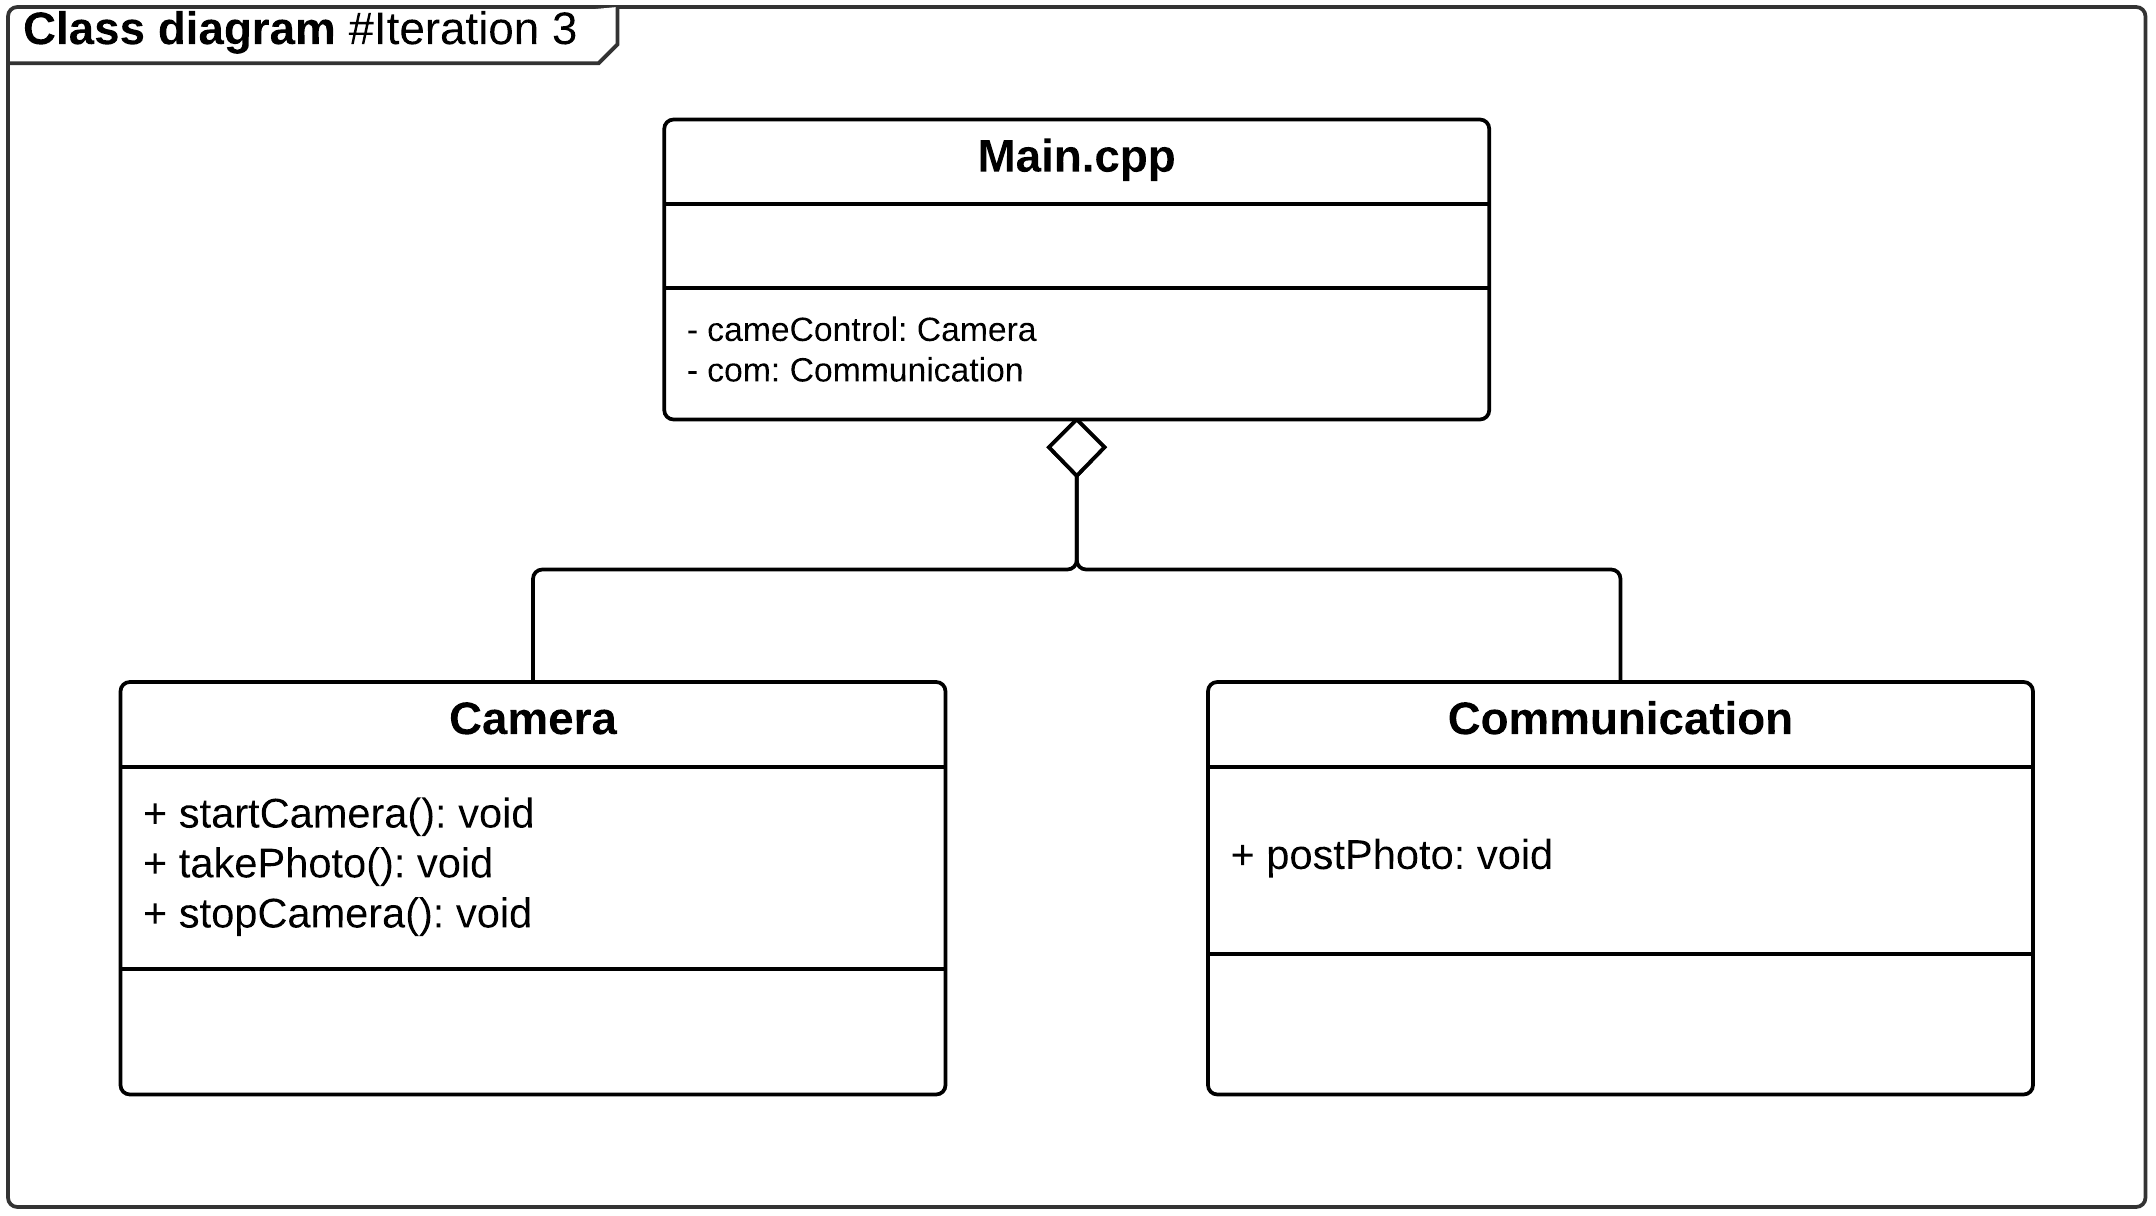
\includegraphics[width=1\textwidth]{Billeder/klasse_diagrammer/classdiagram_iteration3.png}
	\vspace{-0.5cm}
	\caption{Klassediagram \#iteration 3}
	\label{fig:classDiagram_iteration3}
\end{figure}

\textbf{Main.cpp} \\
Main.cpp filen bruges til at oprette objekter af de Anti collision klassen og til at kalde dens tilhørende funktioner.

\textbf{Camera} \\
Klassen eneste funktion er at kontrollere afstanden til eventuelle objekter foran dronen. 





